\documentclass[11pt]{amsart}
\usepackage[utf8]{inputenc}
\usepackage{xcolor}
\usepackage{amsmath,amssymb,amsthm}
\usepackage{graphicx}
\usepackage{booktabs}
\usepackage{microtype}
\setlength{\emergencystretch}{2em}
\usepackage[margin=1in]{geometry}
\usepackage[colorlinks=true,linkcolor=blue!50!black,citecolor=blue!50!black,urlcolor=blue!50!black]{hyperref}

\newtheorem{proposition}{Proposition}[section]
\newtheorem{lemma}[proposition]{Lemma}
\theoremstyle{remark}
\newtheorem{remark}[proposition]{Remark}
\theoremstyle{definition}
\newtheorem{definition}[proposition]{Definition}

\renewcommand{\Re}{\operatorname{Re}}
\renewcommand{\Im}{\operatorname{Im}}
\newcommand{\F}{\mathbb F}
\newcommand{\dd}{\,\mathrm{d}}

\title[Prime-side Weil forms with a Davenport--Heilbronn control]{Prime-side Weil forms in finite windows: \\ a numerical Hodge-index test \\ with a Davenport--Heilbronn control}
\author{Vincent P.\,P. No\"el}
\address{Strasbourg, France}
%\email{}   % to be completed by the author
\date{October 2026. Preprint, not peer reviewed.}
\subjclass[2020]{Primary 11M26; Secondary 11G20, 11Y35, 15B05}
\keywords{Weil's explicit formula, Weil positivity, Hodge index theorem, Toeplitz forms, Davenport--Heilbronn function}

\begin{document}

\begin{abstract}
Weil's criterion states that the Riemann Hypothesis is equivalent to the positivity of a quadratic form built from the explicit formula; the analogy with the Castelnuovo--Hodge positivity on the surface $C\times C$ of a curve over a finite field goes back to Weil. We make this dictionary explicit in finite dimension and test it numerically, using the arithmetic coefficients of $-F'/F$, the archimedean term and the pole. For curves over $\F_q$ we prove an elementary inertia count: for a polynomial with the functional equation of a Weil polynomial and distinct roots, the intersection form built from its point counts has exactly $1+r/2$ positive directions, where $r$ is the number of roots off the circle $|\alpha|=\sqrt q$; we check it on $425$ hyperelliptic curves and on $220$ ``fake'' polynomials that verify non-negative integral closed-point counts through degree $200$ but violate the Riemann Hypothesis. For $\zeta$, $L(s,\chi_5)$ and the Davenport--Heilbronn function we compute the corresponding Toeplitz forms on $180$ settings, each audited against the zero side to relative accuracy $10^{-6}$. At relative eigenvalue tolerance $10^{-11}$, the numerical count for the form of $\zeta$ is exactly one positive direction and that of $L(s,\chi_5)$ none in every setting, while the Davenport--Heilbronn form has excess positive directions in $47$ of the $48$ settings whose arithmetic cutoff is about $56$ or more, and none in the $12$ settings that stop near $20$; the number of excess directions depends on the window and is not an invariant. A separate interval certificate gives at least $25$ negative directions in the fixed Davenport--Heilbronn window $a=0.02$, $h=0.005$, $L=1115$, under the stated arithmetic model; the exact negative count remains unresolved. The positivity observed for $\zeta$ is expected from the known verifications of RH and serves as a consistency check; the note claims no progress towards RH.
\end{abstract}

\maketitle

\section{Introduction}

For a curve $C$ of genus $g$ over $\F_q$, Weil proved the Riemann Hypothesis by a positivity statement on the surface $C\times C$: the intersection form on divisors has exactly one positive direction (Castelnuovo--Severi inequality, Hodge index theorem) \cite{Wei48}. For $\zeta$, Weil's criterion \cite{Wei52} asserts that RH is equivalent to the non-negativity of the quadratic functional of the explicit formula; Bombieri~\cite{Bom00} gives a detailed exposition; the analogy with the surface case goes back to Weil. Connes' programme \cite{Con99,CCM25,CvS25} and the Arithmetic Site of Connes--Consani \cite{CC14} seek a geometric setting in which this positivity would follow from structure. On the numerical side, Zhu~\cite{Zhu26} certifies Weil positivity for $\zeta$ in compact windows with rigorous two-sided bounds, and Suzuki~\cite{Suz26} and Kim et al.~\cite{Kim26} realise Weil's form as the quadratic form of a self-adjoint operator.

This note is more modest. It does three things.
\begin{enumerate}
\item It writes the dictionary between $C\times C$ and the explicit formula as an identity between finite matrices: the fibres correspond to the pole, the intersections of Frobenius graphs to prime powers, the self-intersection to the archimedean term, and the orthogonal complement of the fibres to the Toeplitz Gram matrix of the zeros (Propositions~\ref{prop:dict} and~\ref{prop:zeta}). The substance is classical; we make no claim of novelty for it.
\item In the function-field model it proves an exact inertia count for polynomials that satisfy the functional equation but not RH (Proposition~\ref{prop:inertia}), and checks it on $220$ such ``fake'' polynomials whose closed-point counts are non-negative integers through degree $200$. These show that integrality and non-negativity through the tested finite degree range do not imply the Hodge index; no global effectivity theorem for these fakes is claimed.
\item For $\zeta$, $L(s,\chi_5)$ and the Davenport--Heilbronn function $f_{DH}$ it computes the forms from arithmetic coefficients alone, on $180$ settings, with two controls: $L(s,\chi_5)$ (no pole) and $f_{DH}$ (functional equation, no Euler product, zeros off the line).
\end{enumerate}
The positivity of the $\zeta$ form in our windows is not new information: RH is verified up to height $3\cdot10^{12}$~\cite{PT21}, and the much higher zeros are expected to be negligible at our precision for these test functions; no rigorous tail certificate is supplied here. Its role is to validate the prime-side computation. The Davenport--Heilbronn control shows that the same computation, with the same tolerances, detects zeros off the line from the arithmetic coefficients. Unlike~\cite{Zhu26}, the original $180$-setting grid is in floating point and is not certified. A separate interval calculation now gives a certified lower bound in one fixed Davenport--Heilbronn window (Section~\ref{sec:certificate}); it does not certify the full grid.

\section{The function-field model}\label{sec:ff}

Let $C$ be a smooth projective curve of genus $g$ over $\F_q$, with zeta function $Z(u)=P(u)/((1-u)(1-qu))$, $P(u)=\prod_{i=1}^{2g}(1-\alpha_iu)$, and $S_d=\sum_i\alpha_i^d$, so that $N_d=\#C(\F_{q^d})=q^d+1-S_d$; put $S_0=2g$. On $C\times C$ consider the fibres $f_1=\mathrm{pt}\times C$, $f_2=C\times\mathrm{pt}$ and the graphs $\Gamma_n$ of the $n$-th power of Frobenius, $n\ge0$.

\begin{proposition}[classical]\label{prop:dict}
$f_1^2=f_2^2=0$, $f_1\cdot f_2=1$, $\Gamma_n\cdot f_1=1$, $\Gamma_n\cdot f_2=q^n$, $\Gamma_n^2=q^n(2-2g)$ and $\Gamma_m\cdot\Gamma_n=q^{\min(m,n)}N_{|m-n|}$ for $m\ne n$. With $D_n=q^{-n/2}\Gamma_n$ and $D_n^\perp$ the projection of $D_n$ orthogonally to the hyperbolic plane $\langle f_1,f_2\rangle$,
\[
D_m^\perp\cdot D_n^\perp=-q^{-|m-n|/2}S_{|m-n|}\qquad(m,n\ge0).
\]
If $|\alpha_i|=\sqrt q$ for all $i$, with $\alpha_i=\sqrt q\,e^{i\theta_i}$, this is $-\sum_ie^{i(m-n)\theta_i}$: minus the Toeplitz Gram matrix of the Frobenius angles.
\end{proposition}
\begin{proof}
The intersection numbers are standard (e.g.\ \cite{Wei48,Bom73}). Since $f_1\cdot f_2=1$ and $f_i^2=0$, the projection subtracts $(D_m\cdot f_1)(D_n\cdot f_2)+(D_m\cdot f_2)(D_n\cdot f_1)=q^{(n-m)/2}+q^{(m-n)/2}$ from $D_m\cdot D_n=q^{-(m+n)/2}q^{\min(m,n)}N_{|m-n|}=q^{d/2}+q^{-d/2}-q^{-d/2}S_d$ ($d=|m-n|>0$), and $2$ from $D_n^2=2-2g$.
\end{proof}

By the Hodge index theorem the form on $\langle f_1,f_2,D_0,\dots,D_K\rangle$ has exactly one positive direction; by Proposition~\ref{prop:dict} this amounts to $\big(\sum_i\beta_i^{m-n}\big)_{m,n}\succeq0$ with $\beta_i=\alpha_i/\sqrt q$, which for all $K$ is equivalent to $|\beta_i|=1$. Now let $P$ be any real polynomial of degree $2g$ with the functional equation $u^{2g}P(1/(qu))=q^{-g}P(u)$, so that its inverse roots, normalised as $\beta_i=\alpha_i/\sqrt q$, are stable under $\beta\mapsto\bar\beta$ and $\beta\mapsto1/\bar\beta$. Define $S_d$ and the form $M_K$ on $\langle f_1,f_2,D_0,\dots,D_K\rangle$ by the formulas of Proposition~\ref{prop:dict}.

\begin{proposition}\label{prop:inertia}
Assume the $\beta_i$ are distinct, let $r$ be the number of $i$ with $|\beta_i|\ne1$, and let $K+1\ge2g$. Then $M_K$ has exactly $1+r/2$ positive directions.
\end{proposition}
\begin{proof}
$M_K$ is congruent to the orthogonal sum of the hyperbolic plane $\langle f_1,f_2\rangle$, of signature $(1,1)$, and of $-T$, where $T_{mn}=\sum_i\beta_i^{m-n}$. For $x\in\mathbb C^{K+1}$ put $u_i(x)=\sum_mx_m\overline{\beta_i}^{\,m}$. Then the contribution of $\beta_i$ to $x^*Tx$ is $\overline{u_i(x)}u_{1/\overline{\beta_i}}(x)$. If $|\beta_i|=1$, this is $|u_i|^2$. The off-circle nodes come in pairs $\{\beta,1/\bar\beta\}$, and the two terms of a pair add up to $\bar u v+\bar v u=2\Re(\bar u v)$ with $u=u_\beta$, $v=u_{1/\bar\beta}$, a form of signature $(1,1)$. Since the $2g\le K+1$ nodes are distinct, the linear forms $u_i$ are independent (Vandermonde), and by Sylvester's law of inertia $T$ has $2g-r+r/2$ positive and $r/2$ negative directions. Hence $-T$ has $r/2$ positive directions and $M_K$ has $1+r/2$.
\end{proof}

\begin{remark}
The real $\beta$ off the circle are covered by the same argument (the pair is $\{\beta,1/\beta\}$). Without distinct nodes the count is an upper bound.
\end{remark}

\subsection*{Numerical check} We used $425$ hyperelliptic curves $y^2=f(x)$ with random $f$ over $\F_3$, $\F_5$, $\F_7$ and $1\le g\le8$ (25 curves for each of the $17$ pairs $(q,g)$ used: $g\le4$ for $q=7$, $g\le5$ for $q=5$, $g\le8$ for $q=3$), with $P$ reconstructed from point counts, and $220$ \emph{fake} polynomials: integer polynomials of degree $2g\in\{2,4\}$ over $q\in\{3,5\}$ with the functional equation, whose numbers of closed points of each degree $d\le200$, computed from the $S_d$ by M\"obius inversion, are non-negative integers, but which violate RH. The full form $M_{2g+1}$ has exactly one positive direction for all $425$ curves; for the fakes it has $2$ positive directions in the $101$ cases with $r=2$ and $3$ in the $119$ cases with $r=4$, as predicted. The fakes satisfy the functional equation and the tested finite effectivity conditions through degree $200$; what they lack is what makes the Hodge index hold on a genuine surface, namely Riemann--Roch together with an ample class.

\section{The prime-side form for $L$-functions}\label{sec:L}

Let $\chi_5$ be the character mod $5$ with $\chi_5(2)=i$, and let $F$ be $\zeta$, $L(s,\chi_5)$ or the Davenport--Heilbronn function
\[
f_{DH}(s)=\tfrac12(1-i\xi)L(s,\chi_5)+\tfrac12(1+i\xi)L(s,\bar\chi_5),
\]
with $\xi=(\sqrt{10-2\sqrt5}-2)/(\sqrt5-1)$ \cite{DH36}. Write the non-trivial zeros as $\rho=\frac12+i\gamma_\rho$, with $\gamma_\rho\in\mathbb C$ ($\gamma_\rho$ is real exactly when $\rho$ is on the critical line).

\emph{Test function.} Fix $a>0$ and $\varphi(u)=\cos^4(\pi u/2a)$ for $|u|\le a$, $0$ otherwise; $g=\varphi*\varphi$ has support $[-2a,2a]$ and $\hat g=\hat\varphi^2\ge0$ on $\mathbb R$, where $\hat f(r)=\int f(u)e^{iru}\dd u$. For a step $h>0$ define
\[
t_n=\sum_\rho\hat g(\gamma_\rho)e^{i\gamma_\rho nh}\qquad(n\ge0),\qquad t_{-n}=\overline{t_n},\qquad G_L=(t_{j-k})_{0\le j,k<L}.
\]
By the Guinand--Weil explicit formula \cite{Wei52,Bom00}, $t_n$ is computed \emph{without any zero}: it is the sum of an arithmetic term $-\sum_{m\ge2}\big[c(m)g(\log m-nh)+\overline{c(m)}g(-\log m-nh)\big]/\sqrt m$, where $-F'/F=\sum c(m)m^{-s}$, which involves only $m\le e^{nh+2a}$; an archimedean term $\frac1\pi\int_0^\infty\hat g(r)\cos(rnh)\big[\log(q/\pi)+\Re\psi(\frac{1/2+\mathfrak a}2+\frac{ir}2)\big]\dd r$ with conductor $q$ and parity $\mathfrak a$; and, for $\zeta$, the pole term $2\hat g(i/2)\cosh(nh/2)$. Thus $G_L$ uses arithmetic indices up to $X=e^{Lh+2a}$. For $\zeta$ and $L(s,\chi_5)$ the coefficients $c(m)$ are supported on prime powers. For $f_{DH}$ they need not be: with the above normalisation $c(6)=(1+\xi^2)\log6\ne0$. The term ``prime side'' therefore denotes the arithmetic side of the explicit formula, not a prime-power-only sum for the control function.

\begin{lemma}\label{lem:psd}
If every $\gamma_\rho$ is real, the convergent sum
\[
G_L=\sum_\rho\hat g(\gamma_\rho)v_\rho v_\rho^*\succeq0,
\qquad v_\rho=(e^{i\gamma_\rho jh})_{0\le j<L},
\]
is positive semidefinite. The same is true of every finite sum restricted to real ordinates.

For an off-line pair $\gamma_\pm=\gamma_0\pm i\delta$, $\delta>0$, put $w=\hat g(\gamma_-)$, $x=v_{\gamma_-}$ and $y=v_{\gamma_+}$. Its contribution is
\[
H_{\rm pair}=wxy^*+\bar w yx^*
=U\begin{pmatrix}0&w\\\bar w&0\end{pmatrix}U^*,\qquad U=[x,y].
\]
If $w\ne0$ and $\operatorname{rank}U=2$, this contribution has one positive and one negative direction. After compression by a matrix $P$, the same statement requires $\operatorname{rank}(P^*U)=2$. A quadruplet has signature $(2,2)$ only when its four vectors, before or after the stated compression, remain independent and the two weights are nonzero.
\end{lemma}
\begin{proof}
The real-ordinate terms have nonnegative weights and are positive semidefinite. For the pair, $\hat g(\gamma_+)=\overline{\hat g(\gamma_-)}$ because $g$ is real and even. Its displayed coefficient matrix has eigenvalues $\pm|w|$. Full column rank of $U$, or of $P^*U$ after compression, preserves this nonzero inertia; apply the same argument to the two blocks of a quadruplet.
\end{proof}

\begin{remark}\label{rem:approx}
Discarding small weights does not justify exact positivity of the original form. If a positive semidefinite truncated form $G_L^{(R)}$ satisfies $\|G_L-G_L^{(R)}\|_2\le\varepsilon$, then $\lambda_{\min}(G_L)\ge-\varepsilon$. Exact positivity follows, for example, if $\lambda_{\min}(G_L^{(R)})>\varepsilon$. Likewise, adding a positive background or projecting away vectors can conceal the negative direction of a pair; its contribution alone does not determine the inertia of the complete compressed form.
\end{remark}

\emph{The virtual intersection form of $\zeta$.} Put $c_2=\hat g(i/2)>0$, $a_n=\sqrt{c_2}\,e^{-nh/2}$, $b_n=\sqrt{c_2}\,e^{nh/2}$ and define, on a space with basis $f_1,f_2,D_0,\dots,D_{L-1}$,
\[
M_L=\begin{pmatrix}0&1&a^{T}\\1&0&b^{T}\\a&b&ab^{T}+ba^{T}-G_L\end{pmatrix}.
\]
This is the image of Proposition~\ref{prop:dict} under the dictionary: $(ab^T+ba^T)_{jk}=2c_2\cosh((j-k)h/2)$ is the pole part of $t_{j-k}$ (the fibres), the arithmetic part of $t$ plays the role of $N_{|m-n|}$, and the archimedean part that of the genus term. For $L(s,\chi_5)$ and $f_{DH}$, which have no pole, the form is $M_L=-G_L$.

\begin{proposition}\label{prop:zeta}
The number of positive eigenvalues of $M_L$ equals $1+\nu(G_L)$ for $\zeta$, and $\nu(G_L)$ for $L(s,\chi_5)$ and $f_{DH}$, where $\nu(G_L)$ is the number of negative eigenvalues of $G_L$. In particular, the ``virtual Hodge index'' of $\zeta$ (exactly one positive direction) is equivalent to the finite-window Weil positivity $G_L\succeq0$.
\end{proposition}
\begin{proof}
Projecting $D_j$ orthogonally to $\langle f_1,f_2\rangle$ subtracts $a_jb_k+b_ja_k$, so $M_L$ is congruent to the orthogonal sum of a hyperbolic plane and $-G_L$; apply Sylvester's law of inertia.
\end{proof}

Proposition~\ref{prop:zeta} shows that the geometric language adds no information to Weil positivity; it only places the pole where the fibres are. The interest of the computation below lies in the controls.

\section{Computations}\label{sec:num}

\emph{Settings.} $a\in\{0.02,0.04,0.08,0.16\}$, $h\in\{0.005,0.01,0.02\}$, and for each pair five window lengths $L$ with $X=e^{Lh+2a}$ between $16.8$ and $2996$: $60$ settings per function, $180$ in all.

\emph{Audit.} For every setting, the traces $t_0,\dots,t_L$ computed from the primes were compared with the traces computed from lists of zeros ($1070$ zeros of $\zeta$ up to height $1500$; zeros of $L(s,\chi_5)$ and $f_{DH}$ up to height $600$, the latter including $15$ off-line quadruplets, the lowest at $0.8085+85.699i$ and its partners). The relative discrepancy $\max_n|t_n^{\rm primes}-t_n^{\rm zeros}|/\max_n|t_n^{\rm zeros}|$ is at most $10^{-6}$ in all $180$ settings (about $10^{-12}$ for $\zeta$ and $2\cdot10^{-9}$ for the others at $a=0.04$, $h=0.01$, $L=600$).

\emph{Tolerance.} An eigenvalue is counted as positive (negative) if it exceeds (is below) $10^{-11}$ times the largest absolute eigenvalue. The matrices $G_L$ are numerically rank-deficient (eigenvalues at the level $10^{-13}$--$10^{-12}$ for $\zeta$), so the counts are statements at this tolerance. Agreement of two trace computations to $10^{-6}$ is a consistency check, not a sign certificate at a $10^{-11}$ threshold. A rigorous entrywise trace error $\delta$ would imply $\|\widehat G_L-G_L\|_2\le L\delta$; eigenvalue signs would then require margins exceeding that error and the eigensolver error.

\begin{table}[h]
\centering\small
\begin{tabular}{lccc}
\toprule
 & settings & positive directions of $M_L$ & excess over $1$ ($\zeta$) or $0$\\
\midrule
$\zeta$ & 60 & exactly $1$ in $60/60$ & none\\
$L(s,\chi_5)$ & 60 & $0$ in $60/60$ & none\\
$f_{DH}$ & 60 & $0$ in $12/12$ with $X\le20.3$; $\ge2$ in $47/48$ with $X\ge55.7$ & even in $59/60$\\
\bottomrule
\end{tabular}
\caption{Numerical signature over $180$ audited settings, at relative eigenvalue tolerance $10^{-11}$. These counts alone are not sign certificates.}\label{tab:sig}
\end{table}

\begin{figure}[t]
\centering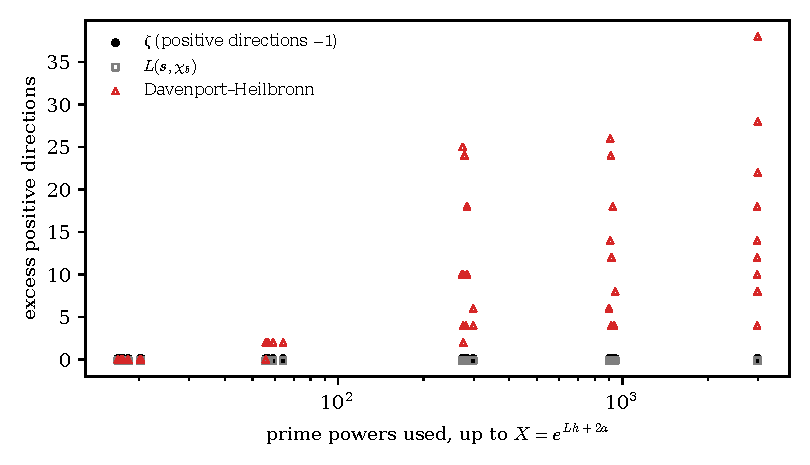
\includegraphics[width=0.8\textwidth]{art2_fig1.pdf}
\caption{Excess positive directions of $M_L$ in the $180$ settings, against the arithmetic cutoff $X$. $\zeta$ and $L(s,\chi_5)$ are slightly offset vertically for visibility.}\label{fig:count}
\end{figure}

\begin{figure}[t]
\centering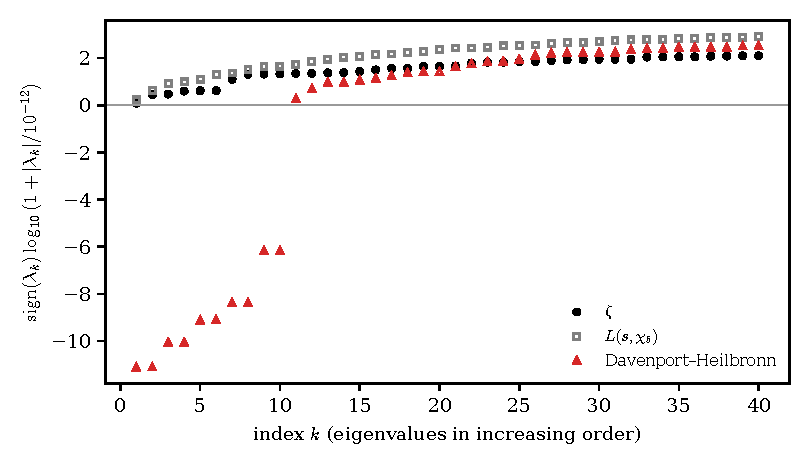
\includegraphics[width=0.8\textwidth]{art2_fig2.pdf}
\caption{The $40$ smallest eigenvalues of $G_L$ for $a=0.04$, $h=0.01$, $L=600$ ($X=439$), on a signed logarithmic scale. $\zeta$: $\lambda_{\min}=2.3\cdot10^{-13}$ (numerical zero). $f_{DH}$: ten negative eigenvalues in five nearly equal pairs, the lowest $-0.1265$, against $\lambda_{\max}=0.741$.}\label{fig:eig}
\end{figure}

\emph{Results.} Table~\ref{tab:sig} and Figures~\ref{fig:count}--\ref{fig:eig} summarise the computation. The signature of the $\zeta$ form is that of a surface, and $L(s,\chi_5)$ has no positive direction, in all settings. The Davenport--Heilbronn form has no excess direction in the $12$ settings with $X\le20.3$, and excess directions in $47$ of the $48$ settings with $X\ge55.7$ (the exception is $a=0.02$, $h=0.02$, $X=55.7$); no setting falls between $20.3$ and $55.7$, so the threshold is only bracketed. Its negative eigenvalues come in nearly equal pairs (Figure~\ref{fig:eig}), as Lemma~\ref{lem:psd} suggests for quadruplets $\{\rho,1-\bar\rho,\bar\rho,1-\rho\}$; the odd numerical count ($25$, at $a=0.02$, $h=0.005$, $X\approx275$) is revisited below through a certified lower bound.


\subsection*{An interval certificate for one DH window}\label{sec:certificate}
We now revisit the odd numerical count $25$ at $a=1/50$, $h=1/200$, $L=1115$. This is a separate validated computation, not a certification of the $180$-setting grid. No zero enters its construction. Arithmetic coefficients of DH are formed from the exact radical $\xi$ and logarithms in interval arithmetic (60 decimal digits), and $g$ is evaluated from its closed trigonometric convolution formula.

For $\sigma_\Gamma=3/4$ and $t=nh$, the integral representation of the digamma function \cite[5.9.16]{DLMF} gives the exact physical-space archimedean term
\[
A(t)=(\log(5/\pi)-\gamma_E)g(t)+
\int_0^\infty\frac{e^{-u}g(t)-\frac12e^{-\sigma_\Gamma u}
[g(t+u/2)+g(t-u/2)]}{1-e^{-u}}\,\mathrm du.
\]
The singularity at $u=0$ is removable. For $B=2t+4a$ the tail equals $-g(t)\log(1-e^{-B})$. If $t>2a$, the entire term instead reduces to
\[
A(t)=-\int_{-2a}^{2a}g(x)
\frac{e^{-2\sigma_\Gamma(t-x)}}{1-e^{-2(t-x)}}\,\mathrm dx.
\]
The quadrature uses enclosed Gauss--Legendre nodes and weights of order $16$, with analytic Cauchy bounds on each smooth branch. A panel of width $\ell$ with analyticity radius $r$ and complex majorant $M$ has error at most $\ell^{33}(16!)^4M/(33(32!)^2r^{32})$. The original Fourier quadrature is used only for comparison. Complete majorants, interval endpoints and the certificate are supplied in the accompanying files \texttt{PREUVE\_NORME\_V636.md}, \texttt{v636\_traces\_intervalles.json} and \texttt{v636\_temoin\_negatif.npz}.

Let $\delta_k$ bound the error of trace $k$ about its binary64 centre. Toeplitz structure gives
\[
\|G-\widehat G\|_2\le
\left(L\delta_0^2+2\sum_{k=1}^{L-1}(L-k)\delta_k^2\right)^{1/2}
\le1.757\cdot10^{-16}.
\]
The maximum quadrature remainder is below $6.855\cdot10^{-25}$. The Frobenius discrepancy between the old Fourier centres and the physical centres is about $4.281\cdot10^{-14}$; this measured discrepancy is not used as the certified error bound.

\begin{proposition}[Validated lower bound in the fixed window]
Under the documented interval arithmetic and standard binary64 rounding model, $G_{1115}$ for DH has at least $25$ negative directions.
\end{proposition}
\begin{proof}[Certificate]
A numerical eigensolver proposes a matrix $V$ with $25$ columns. Its entries are then treated as exact dyadic numbers; their column norms squared are enclosed and checked below $2$. We compute $V^T\widehat GV$ and bound both matrix products using the deterministic factor $\gamma_{2L+2}=(2L+2)u/(1-(2L+2)u)$, $u=2^{-53}$, with outward scalar rounding \cite{HM19}. The trace uncertainty contributes at most $2\|G-\widehat G\|_2$ to each entry. The resulting entry error is at most $2.639\cdot10^{-13}$. Adding these errors to the Gershgorin row sums gives a rightmost bound below $-6.087\cdot10^{-9}$ for the exact compression $V^TGV$. It is negative definite, hence $V$ has full column rank and $G$ has at least $25$ negative directions. The approximate eigenvectors merely propose the witness; their eigenvalue residuals are not used as a proof of the count.
\end{proof}
The hypothesis on binary64 products excludes overflow and significant underflow and uses the usual deterministic rounding model. The computation supplies a lower bound, not an exact inertia: no certificate of positivity for the complementary subspace is given. In particular, an odd lower bound does not contradict the two negative directions of an isolated quadruplet; adding background terms or compressing can conceal one of its directions.

\emph{The count is not an invariant.} At fixed $X$ the number of excess directions of $f_{DH}$ depends on $h$ and $a$: for $a=0.02$ and $X\approx3000$ it is $38$, $18$ and $12$ for $h=0.005$, $0.01$, $0.02$. It is therefore not a count of off-line zeros: how many quadruplets a window ``sees'' depends on the resolution $Lh$ and on the decay of $\hat g$ at the relevant heights. A simple threshold rule on the weights $|\hat g(\gamma_\rho)|$ reproduces the observed counts in only $5$--$10\%$ of the settings; we have no exact rule. The absence of excess directions for $\zeta$ and $L(s,\chi_5)$ and their detection for $f_{DH}$ refer to this finite grid and its chosen tolerance, not to all continuous parameters.

\section{Discussion}

For $\zeta$, Proposition~\ref{prop:zeta} reduces the virtual Hodge index to Weil positivity in a window, and the computation is consistent with known verifications of RH in the relevant height range; it is a consistency check of the pipeline, not evidence for RH. Three points may nonetheless be useful. First, the dictionary is exact in finite dimension, including the pole, which plays the role of the fibres and accounts for the single positive direction. Second, in the function-field model the fake polynomials of Section~\ref{sec:ff} show that the functional equation and non-negative integral counts in the tested finite degree range do not force the signature; on a genuine surface it is forced by Riemann--Roch and an ample class, and no construction enforcing the corresponding positivity for $\zeta$ is supplied here. Such a structural step is the gap addressed by the programmes of \cite{Con99,CC14,CCM25}. Third, the Davenport--Heilbronn control shows that the prime-side computation, with modest resources (arithmetic coefficients indexed by $m\le57$ at $a=0.04$, $h=0.01$), detects the off-line zeros of $f_{DH}$ (the lowest at height $\approx86$), while the number of excess directions is window-dependent.

\subsection*{Acknowledgements and disclosure}
The original computations and draft used Anthropic's Claude. The V6.34 audit and revisions, including the coefficient-support and compression statements, and the V6.36 interval certificate were assisted by OpenAI's ChatGPT. Final mathematical verification and responsibility for submission rest with the author; the note has not been independently refereed. Code and data are available from the author.

\enlargethispage{2\baselineskip}
\begin{thebibliography}{99}
\bibitem{DLMF} NIST Digital Library of Mathematical Functions, \S5.9, equation 5.9.16, \url{https://dlmf.nist.gov/5.9#E16}.
\bibitem{HM19} N. J. Higham, T. Mary, \emph{A New Approach to Probabilistic Rounding Error Analysis}, SIAM J. Sci. Comput. 41 (2019), A2815--A2835. Only the standard deterministic rounding model is used here. \url{https://doi.org/10.1137/18M1226312}.

\bibitem{Bom73} E. Bombieri, \emph{Counting points on curves over finite fields (d'apr\`es S. A. Stepanov)}, S\'eminaire Bourbaki, exp.~430 (1973).
\bibitem{Bom00} E. Bombieri, \emph{Remarks on Weil's quadratic functional in the theory of prime numbers, I}, Rend. Mat. Acc. Lincei (9) 11 (2000), 183--233.
\bibitem{CC14} A. Connes, C. Consani, \emph{The Arithmetic Site}, C. R. Math. Acad. Sci. Paris 352 (2014), 971--975.
\bibitem{CCM25} A. Connes, C. Consani, H. Moscovici, \emph{Zeta spectral triples}, arXiv:2511.22755 (2025).
\bibitem{Con99} A. Connes, \emph{Trace formula in noncommutative geometry and the zeros of the Riemann zeta function}, Selecta Math. (N.S.) 5 (1999), 29--106.
\bibitem{CvS25} A. Connes, W. D. van Suijlekom, \emph{Quadratic forms, real zeros and echoes of the spectral action}, arXiv:2511.23257 (2025).
\bibitem{DH36} H. Davenport, H. Heilbronn, \emph{On the zeros of certain Dirichlet series}, J. London Math. Soc. 11 (1936), 181--185 and 307--312.
\bibitem{Kim26} T. Kim, Y. Hong, M. Kim, S. Choi, J. Jang, M. Kim, \emph{A numerical realization of Suzuki's Weil-quadratic-form operator}, arXiv:2607.24830 (2026).
\bibitem{PT21} D. J. Platt, T. S. Trudgian, \emph{The Riemann hypothesis is true up to $3\cdot10^{12}$}, Bull. London Math. Soc. 53 (2021), 792--797.
\bibitem{Suz26} M. Suzuki, \emph{Weil's quadratic form via the screw function}, arXiv:2606.09096 (2026).
\bibitem{Wei48} A. Weil, \emph{Sur les courbes alg\'ebriques et les vari\'et\'es qui s'en d\'eduisent}, Hermann, Paris, 1948.
\bibitem{Wei52} A. Weil, \emph{Sur les ``formules explicites'' de la th\'eorie des nombres premiers}, Comm. S\'em. Math. Univ. Lund, vol. suppl\'ementaire (1952), 252--265.
\bibitem{Zhu26} X. Zhu, \emph{Weil positivity in compact windows: a finite reduction, certified two-sided bounds, and a Landau--Widom decay law}, arXiv:2608.24827 (2026).
\end{thebibliography}

\end{document}
